% answers.tex —— 2005 年·普通高等学校招生考试·天津卷·理科 · 参考答案与详细解析片段
% 由 tools/generate_projects.py 依来源总账自 2005/2005_数学真题_天津理科_试题.md + 2005/2005_数学真题_天津理科_解析正文.md + 2005/2005_数学真题_天津理科_答案要点.md 生成，勿手改（改源 MD 后重跑）


\begin{gktip}
固定源 PDF 为印刷页码 266–267 的两页题面，不附官方答案。以下解析均依据固定源独立推导复算；各题配图在 LaTeX 工程中均以 TikZ 纯矢量重绘。
\end{gktip}

\begin{answer}
\gksolhead{1}{}

\textbf{题目}：

设集合 $A = \{x \mid |4x - 1| \geqslant 9, x \in \mathbf{R}\}$，$B = \left\{x \mid \dfrac{x}{x+3} \geqslant 0, x \in \mathbf{R}\right\}$，则 $A \cap B =$\mbox{（　　）}

\begin{gkopts}(1)
\task A．$(-3, -2]$
\task B．$(-3, -2] \cup \left[0, \dfrac{5}{2}\right]$
\task C．$(-\infty, -3] \cup \left[\dfrac{5}{2}, +\infty\right)$
\task D．$(-\infty, -3) \cup \left[\dfrac{5}{2}, +\infty\right)$
\end{gkopts}

\Needspace{4\baselineskip}
\textbf{解析}

\Needspace{5\baselineskip}
解绝对值不等式 $|4x - 1| \geqslant 9$：
\nopagebreak[4]
\[
4x - 1 \geqslant 9 \iff 4x \geqslant 10 \iff x \geqslant \dfrac{5}{2},
\]
\Needspace{5\baselineskip}
或
\nopagebreak[4]
\[
4x - 1 \leqslant -9 \iff 4x \leqslant -8 \iff x \leqslant -2.
\]
故集合 $A = (-\infty, -2] \cup \left[\dfrac{5}{2}, +\infty\right)$．

解分式不等式 $\dfrac{x}{x+3} \geqslant 0$：
\Needspace{5\baselineskip}
原不等式等价于
\nopagebreak[4]
\[
\begin{cases} x(x+3) \geqslant 0, \\ x + 3 \neq 0 \end{cases} \iff x \geqslant 0 \text{ \text{或} } x < -3.
\]
故集合 $B = (-\infty, -3) \cup [0, +\infty)$．

求交集 $A \cap B$：
由于 $(-\infty, -2] \cap (-\infty, -3) = (-\infty, -3)$，
且 $\left[\dfrac{5}{2}, +\infty\right) \cap [0, +\infty) = \left[\dfrac{5}{2}, +\infty\right)$，
\Needspace{5\baselineskip}
其余交叉部分为空集，因此
\nopagebreak[4]
\[
A \cap B = (-\infty, -3) \cup \left[\dfrac{5}{2}, +\infty\right).
\]

故选 D．

\gkanswer{答案：D}

\end{answer}
\begin{answer}
\gksolhead{2}{}

\textbf{题目}：

若复数 $\dfrac{a+3\mathrm{i}}{1+2\mathrm{i}}$（$a \in \mathbf{R}$，$\mathrm{i}$ 为虚数单位）是纯虚数，则实数 $a$ 的值为\mbox{（　　）}

\begin{gkopts}(4)
\task A．$-2$
\task B．$4$
\task C．$-6$
\task D．$6$
\end{gkopts}

\Needspace{4\baselineskip}
\textbf{解析}

\Needspace{5\baselineskip}
将复数分子分母同乘以分母的共轭复数 $1 - 2\mathrm{i}$：
\nopagebreak[4]
\[
\begin{aligned}
\dfrac{a+3\mathrm{i}}{1+2\mathrm{i}} &= \dfrac{(a+3\mathrm{i})(1-2\mathrm{i})}{(1+2\mathrm{i})(1-2\mathrm{i})} \\
&= \dfrac{a - 2a\mathrm{i} + 3\mathrm{i} - 6\mathrm{i}^2}{1 - 4\mathrm{i}^2} \\
&= \dfrac{(a+6) + (3-2a)\mathrm{i}}{5} \\
&= \dfrac{a+6}{5} + \dfrac{3-2a}{5}\mathrm{i}.
\end{aligned}
\]
\Needspace{5\baselineskip}
由题意，该复数是纯虚数，则其满足实部为 $0$ 且虚部不为 $0$：
\nopagebreak[4]
\[
\begin{cases} \dfrac{a+6}{5} = 0, \\ \dfrac{3-2a}{5} \neq 0 \end{cases} \implies a = -6.
\]
当 $a = -6$ 时，虚部为 $\dfrac{3 - 2(-6)}{5} = 3 \neq 0$，符合题意．

故选 C．

\gkanswer{答案：C}

\end{answer}
\begin{answer}
\gksolhead{3}{}

\textbf{题目}：

给出下列三个命题：
① 若 $a \geqslant b > -1$，则 $\dfrac{a}{1+a} \geqslant \dfrac{b}{1+b}$；
② 若正整数 $m$ 和 $n$ 满足 $m \leqslant n$，则 $\sqrt{m(n-m)} \leqslant \dfrac{n}{2}$；
③ 设 $P(x_1, y_1)$ 为圆 $O_1: x^2 + y^2 = 9$ 上任一点，圆 $O_2$ 以 $Q(a, b)$ 为圆心且半径为 $1$．当 $(a - x_1)^2 + (b - y_1)^2 = 1$ 时，圆 $O_1$ 与圆 $O_2$ 相切．
其中假命题的个数为\mbox{（　　）}

\begin{gkopts}(4)
\task A．$0$
\task B．$1$
\task C．$2$
\task D．$3$
\end{gkopts}

\Needspace{4\baselineskip}
\textbf{解析}

逐项考查各命题：

对于命题 ①：
考虑函数 $f(t) = \dfrac{t}{1+t} = 1 - \dfrac{1}{1+t}$．
当 $t > -1$ 时，$1+t > 0$，函数 $f(t)$ 在 $(-1, +\infty)$ 上严格单调递增．
因为 $a \geqslant b > -1$，所以 $f(a) \geqslant f(b)$，即 $\dfrac{a}{1+a} \geqslant \dfrac{b}{1+b}$ 恒成立，命题 ① 为真命题．

对于命题 ②：
因为 $m, n \in \mathbf{N}^*$ 且 $m \leqslant n$，所以 $m \geqslant 0$，$n - m \geqslant 0$．
\Needspace{5\baselineskip}
由基本不等式 $\sqrt{xy} \leqslant \dfrac{x+y}{2}$（当且仅当 $x = y$ 时取等号）：
\nopagebreak[4]
\[
\sqrt{m(n-m)} \leqslant \dfrac{m + (n-m)}{2} = \dfrac{n}{2}.
\]
命题 ② 为真命题．

对于命题 ③：
圆 $O_1: x^2 + y^2 = 9$ 的圆心为 $(0, 0)$，半径 $R = 3$．
圆 $O_2$ 的圆心为 $Q(a, b)$，半径 $r = 1$．
条件 $(a - x_1)^2 + (b - y_1)^2 = 1$ 表示点 $P(x_1, y_1)$ 到圆心 $Q(a, b)$ 的距离为 $1$，即点 $P$ 落在圆 $O_2$ 上．
又点 $P$ 在圆 $O_1$ 上，因此点 $P$ 是圆 $O_1$ 与圆 $O_2$ 的一个公共点．
但这仅说明两圆有交点，两圆可以相交，不一定相切．
例如取 $Q(3, 0)$，则圆心距 $d = |O_1Q| = 3$．
由于两圆半径分别为 $R = 3, r = 1$，满足 $|R - r| = 2 < d < R + r = 4$，此时两圆相交而非相切，但点 $P(3, 0)$ 在两圆上且满足该方程．
因此命题 ③ 为假命题．

综上所述，假命题仅有 ③，共 $1$ 个．

故选 B．

\gkanswer{答案：B}

\end{answer}
\begin{answer}
\gksolhead{4}{}

\textbf{题目}：

设 $\alpha, \beta, \gamma$ 为平面，$m, n, l$ 为直线，则 $m \perp \beta$ 的一个充分条件是\mbox{（　　）}

\begin{gkopts}(1)
\task A．$\alpha \perp \beta, \alpha \cap \beta = l, m \perp l$
\task B．$\alpha \cap \gamma = m, \alpha \perp \gamma, \beta \perp \gamma$
\task C．$\alpha \perp \gamma, \beta \perp \gamma, m \perp \alpha$
\task D．$n \perp \alpha, n \perp \beta, m \perp \alpha$
\end{gkopts}

\Needspace{4\baselineskip}
\textbf{解析}

逐个选项分析：

A 选项：若 $\alpha \perp \beta, \alpha \cap \beta = l, m \perp l$．若直线 $m$ 不在平面 $\alpha$ 内（例如 $m$ 在平面 $\beta$ 内且垂直于交线 $l$），则 $m \perp \beta$ 不成立．必须附加“$m \subset \alpha$”条件，故 A 不是充分条件．

B 选项：若 $\alpha \cap \gamma = m, \alpha \perp \gamma, \beta \perp \gamma$．两个平面同时垂直于第三个平面，它们的交线平行于第三个平面的垂线，但直线 $m$ 垂直于 $\gamma$ 并不意味着 $m$ 垂直于 $\beta$（例如直角三棱柱中的侧棱垂直于底面，但不垂直于侧面），故 B 错误．

C 选项：若 $\alpha \perp \gamma, \beta \perp \gamma, m \perp \alpha$．垂直于同一平面的两个平面 $\alpha, \beta$ 可以平行也可以相交．若 $\alpha$ 与 $\beta$ 相交，则垂直于 $\alpha$ 的直线 $m$ 与平面 $\beta$ 可以斜交或平行，不一定垂直，故 C 错误．

D 选项：由 $n \perp \alpha$ 且 $n \perp \beta$，根据垂直于同一直线的两个平面互相平行，得 $\alpha \parallel \beta$．
又已知 $m \perp \alpha$，由垂直于两平行平面之一的直线必垂直于另一个平面，必有 $m \perp \beta$．
因此 D 选项是 $m \perp \beta$ 的充分条件．

故选 D．

\gkanswer{答案：D}

\end{answer}
\begin{answer}
\gksolhead{5}{}

\textbf{题目}：

设双曲线以椭圆 $\dfrac{x^2}{25} + \dfrac{y^2}{9} = 1$ 长轴的两个端点为焦点，其准线过椭圆的焦点，则双曲线的渐近线的斜率为\mbox{（　　）}

\begin{gkopts}(2)
\task A．$\pm 2$
\task B．$\pm \dfrac{4}{3}$
\task C．$\pm \dfrac{1}{2}$
\task D．$\pm \dfrac{3}{4}$
\end{gkopts}

\Needspace{4\baselineskip}
\textbf{解析}

对于椭圆 $\dfrac{x^2}{25} + \dfrac{y^2}{9} = 1$：
长半轴长 $a_e = 5$，短半轴长 $b_e = 3$，半焦距 $c_e = \sqrt{a_e^2 - b_e^2} = \sqrt{25 - 9} = 4$．
长轴端点为 $(\pm 5, 0)$，焦点为 $(\pm 4, 0)$．

由题意，双曲线以长轴端点 $(\pm 5, 0)$ 为焦点，故双曲线的半焦距 $c_h = 5$，焦点在 $x$ 轴上．
其准线过椭圆的焦点 $(\pm 4, 0)$，故双曲线的准线方程为 $x = \pm 4$．
\Needspace{5\baselineskip}
根据双曲线的准线公式 $x = \pm \dfrac{a_h^2}{c_h}$，得：
\nopagebreak[4]
\[
\dfrac{a_h^2}{5} = 4 \implies a_h^2 = 20.
\]
\Needspace{5\baselineskip}
因此
\nopagebreak[4]
\[
b_h^2 = c_h^2 - a_h^2 = 25 - 20 = 5.
\]
双曲线的渐近线方程为 $y = \pm \dfrac{b_h}{a_h} x$．
\Needspace{5\baselineskip}
其斜率为
\nopagebreak[4]
\[
\pm \dfrac{b_h}{a_h} = \pm \sqrt{\dfrac{5}{20}} = \pm \dfrac{1}{2}.
\]

故选 C．

\gkanswer{答案：C}

\end{answer}
\begin{answer}
\gksolhead{6}{}

\textbf{题目}：

从集合 $\{1, 2, 3, \cdots, 11\}$ 中任选两个元素作为椭圆方程 $\dfrac{x^2}{m^2} + \dfrac{y^2}{n^2} = 1$ 中的 $m$ 和 $n$，则能组成落在矩形区域 $B = \{(x, y) \mid |x| < 11 \text{ \text{且} } |y| < 9\}$ 内的椭圆个数为\mbox{（　　）}

\begin{gkopts}(4)
\task A．$43$
\task B．$72$
\task C．$86$
\task D．$90$
\end{gkopts}

\Needspace{4\baselineskip}
\textbf{解析}

椭圆方程为 $\dfrac{x^2}{m^2} + \dfrac{y^2}{n^2} = 1$．
因为是从集合 $\{1, 2, 3, \cdots, 11\}$ 中任选两个元素作为 $m$ 和 $n$，所以 $m \neq n$（若 $m = n$，则方程表示圆而非椭圆）．
椭圆上的任意点 $(x, y)$ 满足 $|x| \leqslant m$ 且 $|y| \leqslant n$．
\Needspace{5\baselineskip}
要使整个椭圆落在矩形区域 $B = \{(x, y) \mid |x| < 11 \text{ \text{且} } |y| < 9\}$ 内，必须且只需椭圆在坐标轴上的顶点落在矩形内部，即：
\nopagebreak[4]
\[
\begin{cases} m < 11, \\ n < 9. \end{cases}
\]
因为 $m, n \in \{1, 2, 3, \cdots, 11\}$，所以：
\begin{itemize}
\item $m$ 可以取 $\{1, 2, 3, \cdots, 10\}$ 中的任意一个整数，共 $10$ 种取法；
\item $n$ 可以取 $\{1, 2, 3, \cdots, 8\}$ 中的任意一个整数，共 $8$ 种取法．
\end{itemize}
若不考虑 $m \neq n$ 的限制，数对 $(m, n)$ 的选法共有 $10 \times 8 = 80$ 种．
其中满足 $m = n$ 的数对为 $(1, 1), (2, 2), \cdots, (8, 8)$，共 $8$ 种．
\Needspace{5\baselineskip}
由于方程必须表示椭圆，必须排除 $m = n$ 的情况，因此满足条件的椭圆个数为：
\nopagebreak[4]
\[
80 - 8 = 72.
\]

故选 B．

\gkanswer{答案：B}

\end{answer}
\begin{answer}
\gksolhead{7}{}

\textbf{题目}：

某人射击一次击中的概率为 $0.6$，经过 $3$ 次射击，此人至少有两次击中目标的概率为\mbox{（　　）}

\begin{gkopts}(2)
\task A．$\dfrac{81}{125}$
\task B．$\dfrac{54}{125}$
\task C．$\dfrac{36}{125}$
\task D．$\dfrac{27}{125}$
\end{gkopts}

\Needspace{4\baselineskip}
\textbf{解析}

设每次射击击中目标的概率为 $p = 0.6$，未击中的概率为 $q = 1 - 0.6 = 0.4$．
经过 $3$ 次独立重复射击，击中目标的次数 $X \sim B(3, 0.6)$．
\Needspace{5\baselineskip}
“至少有两次击中目标”包含击中 $2$ 次和击中 $3$ 次两种互斥情况：
\nopagebreak[4]
\[
P(X = 2) = \mathrm{C}_3^2 p^2 q = 3 \times (0.6)^2 \times (0.4) = 3 \times \dfrac{9}{25} \times \dfrac{2}{5} = \dfrac{54}{125},
\]
\nopagebreak[4]
\[
P(X = 3) = \mathrm{C}_3^3 p^3 = (0.6)^3 = \dfrac{27}{125}.
\]
\Needspace{5\baselineskip}
所以至少有两次击中目标的概率为：
\nopagebreak[4]
\[
P(X \geqslant 2) = P(X = 2) + P(X = 3) = \dfrac{54}{125} + \dfrac{27}{125} = \dfrac{81}{125}.
\]

故选 A．

\gkanswer{答案：A}

\end{answer}
\begin{answer}
\gksolhead{8}{}

\textbf{题目}：

要得到函数 $y = \sqrt{2} \cos x$ 的图象，只需将函数 $y = \sqrt{2} \sin\left(2x + \dfrac{\pi}{4}\right)$ 的图象上所有的点的\mbox{（　　）}

\begin{gkopts}(1)
\task A．横坐标缩短到原来的 $\dfrac{1}{2}$ 倍（纵坐标不变），再向左平行移动 $\dfrac{\pi}{8}$ 个单位长度
\task B．横坐标缩短到原来的 $\dfrac{1}{2}$ 倍（纵坐标不变），再向右平行移动 $\dfrac{\pi}{4}$ 个单位长度
\task C．横坐标伸长到原来的 $2$ 倍（纵坐标不变），再向左平行移动 $\dfrac{\pi}{4}$ 个单位长度
\task D．横坐标伸长到原来的 $2$ 倍（纵坐标不变），再向右平行移动 $\dfrac{\pi}{8}$ 个单位长度
\end{gkopts}

\Needspace{4\baselineskip}
\textbf{解析}

目标函数为 $y = \sqrt{2} \cos x = \sqrt{2} \sin\left(x + \dfrac{\pi}{2}\right)$．
已知函数为 $y = \sqrt{2} \sin\left(2x + \dfrac{\pi}{4}\right)$．
分析变换过程：
\Needspace{5\baselineskip}
第一步，将图象上所有点的横坐标伸长到原来的 $2$ 倍（纵坐标不变），即把解析式中的 $x$ 替换为 $\dfrac{1}{2}x$：
\nopagebreak[4]
\[
y = \sqrt{2} \sin\left(2 \cdot \dfrac{1}{2}x + \dfrac{\pi}{4}\right) = \sqrt{2} \sin\left(x + \dfrac{\pi}{4}\right).
\]
\Needspace{5\baselineskip}
第二步，将得到的图象向左平移 $\dfrac{\pi}{4}$ 个单位长度，即把自变量 $x$ 替换为 $x + \dfrac{\pi}{4}$：
\nopagebreak[4]
\[
y = \sqrt{2} \sin\left(\left(x + \dfrac{\pi}{4}\right) + \dfrac{\pi}{4}\right) = \sqrt{2} \sin\left(x + \dfrac{\pi}{2}\right) = \sqrt{2} \cos x.
\]
此时即得到函数 $y = \sqrt{2}\cos x$ 的图象．
对照选项，C 选项表述完全吻合．

故选 C．

\gkanswer{答案：C}

\end{answer}
\begin{answer}
\gksolhead{9}{}

\textbf{题目}：

设 $f^{-1}(x)$ 是函数 $f(x) = \dfrac{1}{2}(a^x - a^{-x})\ (a > 1)$ 的反函数，则使 $f^{-1}(x) > 1$ 成立的 $x$ 的取值范围为\mbox{（　　）}

\begin{gkopts}(2)
\task A．$\left(\dfrac{a^2 - 1}{2a}, +\infty\right)$
\task B．$\left(-\infty, \dfrac{a^2 - 1}{2a}\right)$
\task C．$\left(\dfrac{a^2 - 1}{2a}, a\right)$
\task D．$[a, +\infty)$
\end{gkopts}

\Needspace{4\baselineskip}
\textbf{解析}

因为 $a > 1$，指数函数 $y = a^x$ 在 $\mathbf{R}$ 上单调递增，函数 $y = -a^{-x}$ 在 $\mathbf{R}$ 上也单调递增，
所以函数 $f(x) = \dfrac{1}{2}(a^x - a^{-x})$ 是 $\mathbf{R}$ 上的严格单调递增函数．
根据严格单调函数的反函数具有相同单调性的性质，反函数 $f^{-1}(x)$ 在其定义域 $\mathbf{R}$ 上也是严格单调递增函数．
\Needspace{5\baselineskip}
因此：
\nopagebreak[4]
\[
f^{-1}(x) > 1 \iff x > f(1).
\]
\Needspace{5\baselineskip}
计算 $f(1)$ 的值：
\nopagebreak[4]
\[
f(1) = \dfrac{1}{2}(a^1 - a^{-1}) = \dfrac{1}{2}\left(a - \dfrac{1}{a}\right) = \dfrac{a^2 - 1}{2a}.
\]
所以 $x$ 的取值范围为 $\left(\dfrac{a^2 - 1}{2a}, +\infty\right)$．

故选 A．

\gkanswer{答案：A}

\end{answer}
\begin{answer}
\gksolhead{10}{}

\textbf{题目}：

若函数 $f(x) = \log_a(x^3 - ax)\ (a > 0, a \neq 1)$ 在区间 $\left(-\dfrac{1}{2}, 0\right)$ 内单调递增，则 $a$ 的取值范围是\mbox{（　　）}

\begin{gkopts}(2)
\task A．$\left[\dfrac{1}{4}, 1\right)$
\task B．$\left[\dfrac{3}{4}, 1\right)$
\task C．$\left(\dfrac{9}{4}, +\infty\right)$
\task D．$\left(1, \dfrac{9}{4}\right]$
\end{gkopts}

\Needspace{4\baselineskip}
\textbf{解析}

设内层函数为 $g(x) = x^3 - ax$，外层函数为 $y = \log_a u$．
要使复合函数 $f(x) = \log_a g(x)$ 在区间 $\left(-\dfrac{1}{2}, 0\right)$ 内单调递增，需满足：
1. 对任意 $x \in \left(-\dfrac{1}{2}, 0\right)$，真数恒正，即 $g(x) > 0$；
2. 依据同增异减原则分两种情况讨论底数 $a$：

若 $a > 1$，外层对数函数递增，则要求内层函数 $g(x) = x^3 - ax$ 在 $\left(-\dfrac{1}{2}, 0\right)$ 内单调递增．
求导得 $g'(x) = 3x^2 - a$．
要使 $g'(x) \geqslant 0$ 在 $\left(-\dfrac{1}{2}, 0\right)$ 上恒成立，需 $a \leqslant 3x^2$ 对该区间内任意 $x$ 成立．
由于当 $x \to 0$ 时 $3x^2 \to 0$，这意味着 $a \leqslant 0$，与 $a > 1$ 矛盾．因此 $a > 1$ 不可能．

若 $0 < a < 1$，外层对数函数递减，依据同增异减原则，要求内层函数 $g(x) = x^3 - ax$ 在 $\left(-\dfrac{1}{2}, 0\right)$ 内单调递减．
此时导数满足 $g'(x) = 3x^2 - a \leqslant 0$ 在 $\left(-\dfrac{1}{2}, 0\right)$ 上恒成立．
因为当 $x \in \left(-\dfrac{1}{2}, 0\right)$ 时，$x^2 \in \left(0, \dfrac{1}{4}\right)$，所以 $3x^2 \in \left(0, \dfrac{3}{4}\right)$．
要使 $a \geqslant 3x^2$ 恒成立，只需 $a \geqslant \dfrac{3}{4}$．
再检验真数 $g(x) > 0$：
\Needspace{5\baselineskip}
当 $\dfrac{3}{4} \leqslant a < 1$ 时，对任意 $x \in \left(-\dfrac{1}{2}, 0\right)$：
\nopagebreak[4]
\[
g(x) = x(x^2 - a).
\]
因为 $x < 0$，且 $x^2 < \dfrac{1}{4} < \dfrac{3}{4} \leqslant a \implies x^2 - a < 0$，
所以 $g(x) = x(x^2 - a) > 0$ 恒成立，满足真数大于 $0$ 的要求．
综上所述，$a$ 的取值范围是 $\left[\dfrac{3}{4}, 1\right)$．

故选 B．

\gkanswer{答案：B}

\end{answer}
\begin{answer}
\gksolhead{11}{}

\textbf{题目}：

设 $n \in \mathbf{N}^*$，则 $\mathrm{C}_n^1 + \mathrm{C}_n^2 6 + \mathrm{C}_n^3 6^2 + \cdots + \mathrm{C}_n^n 6^{n-1} = \underline{\hspace{2em}}$．

\Needspace{4\baselineskip}
\textbf{解析}

\Needspace{5\baselineskip}
由二项式定理：
\nopagebreak[4]
\[
(1 + x)^n = \mathrm{C}_n^0 + \mathrm{C}_n^1 x + \mathrm{C}_n^2 x^2 + \cdots + \mathrm{C}_n^n x^n.
\]
\Needspace{5\baselineskip}
令 $x = 6$，得：
\nopagebreak[4]
\[
7^n = 1 + \mathrm{C}_n^1 \cdot 6 + \mathrm{C}_n^2 \cdot 6^2 + \cdots + \mathrm{C}_n^n \cdot 6^n.
\]
\Needspace{5\baselineskip}
移项可得：
\nopagebreak[4]
\[
\mathrm{C}_n^1 \cdot 6 + \mathrm{C}_n^2 \cdot 6^2 + \cdots + \mathrm{C}_n^n \cdot 6^n = 7^n - 1.
\]
\Needspace{5\baselineskip}
两边同除以 $6$，得：
\nopagebreak[4]
\[
\mathrm{C}_n^1 + \mathrm{C}_n^2 6 + \mathrm{C}_n^3 6^2 + \cdots + \mathrm{C}_n^n 6^{n-1} = \dfrac{7^n - 1}{6}.
\]

\gkanswer{答案：$\dfrac{7^n - 1}{6}$。}

\end{answer}
\begin{answer}
\gksolhead{12}{}

\textbf{题目}：

如图，$PA \perp$ 平面 $ABC$，$\angle ACB = 90^\circ$ 且 $PA = AC = BC = a$，则异面直线 $PB$ 与 $AC$ 所成角的正切值等于 $\underline{\hspace{2em}}$．
\nopagebreak[4]
\begin{center}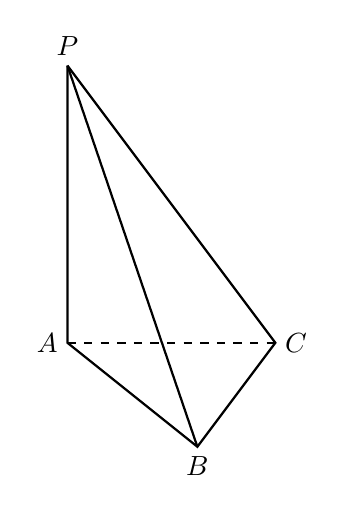
\begin{tikzpicture}[>=stealth, scale=1.1]
  % 顶点坐标
  \coordinate (A) at (0, 0);
  \coordinate (P) at (0, 3.2);
  \coordinate (C) at (2.4, 0);
  \coordinate (B) at (1.5, -1.2);

  % 实线棱
  \draw[thick] (P) -- (A) -- (B) -- (C) -- (P);
  \draw[thick] (P) -- (B);

  % 虚线棱
  \draw[dashed, thick] (A) -- (C);

  % 顶点标签
  \node[above] at (P) {$P$};
  \node[left] at (A) {$A$};
  \node[below] at (B) {$B$};
  \node[right] at (C) {$C$};
\end{tikzpicture}
\end{center}
\nopagebreak[4]
\Needspace{4\baselineskip}
\textbf{解析}

以点 $C$ 为原点，以 $CA$ 为 $x$ 轴，$CB$ 为 $y$ 轴，过点 $C$ 作垂直于底面 $ABC$ 的垂线为 $z$ 轴建立空间直角坐标系．
\Needspace{5\baselineskip}
则各点坐标为：
\nopagebreak[4]
\[
C(0, 0, 0), \quad A(a, 0, 0), \quad B(0, a, 0).
\]
因为 $PA \perp \text{\text{平面} } ABC$ 且 $PA = a$，所以点 $P$ 的坐标为 $(a, 0, a)$．
\Needspace{5\baselineskip}
向量 $\vec{AC}$ 与 $\vec{PB}$ 分别为：
\nopagebreak[4]
\[
\vec{AC} = (0 - a, 0 - 0, 0 - 0) = (-a, 0, 0),
\]
\nopagebreak[4]
\[
\vec{PB} = (0 - a, a - 0, 0 - a) = (-a, a, -a).
\]
模长分别为 $|\vec{AC}| = a$，$|\vec{PB}| = \sqrt{(-a)^2 + a^2 + (-a)^2} = \sqrt{3}a$．
\Needspace{5\baselineskip}
两向量的数量积为：
\nopagebreak[4]
\[
\vec{AC} \cdot \vec{PB} = (-a)(-a) + 0 \cdot a + 0 \cdot (-a) = a^2.
\]
\Needspace{5\baselineskip}
设异面直线 $PB$ 与 $AC$ 所成角为 $\theta$（$0 < \theta \leqslant \dfrac{\pi}{2}$），则：
\nopagebreak[4]
\[
\cos \theta = \dfrac{|\vec{AC} \cdot \vec{PB}|}{|\vec{AC}| |\vec{PB}|} = \dfrac{a^2}{a \cdot \sqrt{3}a} = \dfrac{1}{\sqrt{3}}.
\]
\Needspace{5\baselineskip}
由同角三角函数基本关系式：
\nopagebreak[4]
\[
\sin \theta = \sqrt{1 - \cos^2 \theta} = \sqrt{1 - \dfrac{1}{3}} = \dfrac{\sqrt{6}}{3}.
\]
\Needspace{5\baselineskip}
因此：
\nopagebreak[4]
\[
\tan \theta = \dfrac{\sin \theta}{\cos \theta} = \dfrac{\sqrt{6}/3}{\sqrt{3}/3} = \sqrt{2}.
\]

\gkanswer{答案：$\sqrt{2}$。}

\end{answer}
\begin{answer}
\gksolhead{13}{}

\textbf{题目}：

在数列 $\{a_n\}$ 中，$a_1 = 1$，$a_2 = 2$，且 $a_{n+2} - a_n = 1 + (-1)^n\ (n \in \mathbf{N}^*)$，则 $S_{100} = \underline{\hspace{2em}}$．

\Needspace{4\baselineskip}
\textbf{解析}

已知递推关系式 $a_{n+2} - a_n = 1 + (-1)^n$：
当 $n$ 为奇数时，$(-1)^n = -1$，得 $a_{n+2} - a_n = 1 - 1 = 0$，
即奇数项满足 $a_1 = a_3 = a_5 = \cdots = a_{99} = 1$；
当 $n$ 为偶数时，$(-1)^n = 1$，得 $a_{n+2} - a_n = 1 + 1 = 2$，
即偶数项是首项 $a_2 = 2$、公差 $d = 2$ 的等差数列，$a_{2k} = 2 + (k-1) \times 2 = 2k$．
\Needspace{5\baselineskip}
求 $S_{100}$ 即求前 $100$ 项的和，将奇数项与偶数项分开求和：
\nopagebreak[4]
\[
S_{100} = \sum_{k=1}^{50} a_{2k-1} + \sum_{k=1}^{50} a_{2k}.
\]
\Needspace{5\baselineskip}
奇数项部分共有 $50$ 项，每项均为 $1$：
\nopagebreak[4]
\[
\sum_{k=1}^{50} a_{2k-1} = 50 \times 1 = 50.
\]
\Needspace{5\baselineskip}
偶数项部分共有 $50$ 项，首项为 $2$，末项为 $a_{100} = 2 \times 50 = 100$：
\nopagebreak[4]
\[
\sum_{k=1}^{50} a_{2k} = \dfrac{50 \times (2 + 100)}{2} = 50 \times 51 = 2550.
\]
\Needspace{5\baselineskip}
两部分相加：
\nopagebreak[4]
\[
S_{100} = 50 + 2550 = 2600.
\]

\gkanswer{答案：$2600$。}

\end{answer}
\begin{answer}
\gksolhead{14}{}

\textbf{题目}：

在直角坐标系 $xOy$ 中，已知点 $A(0, 1)$ 和点 $B(-3, 4)$，若点 $C$ 在 $\angle AOB$ 的平分线上且 $|\vec{OC}| = 2$，则 $\vec{OC} = \underline{\hspace{2em}}$．

\Needspace{4\baselineskip}
\textbf{解析}

点 $A(0, 1)$，向量 $\vec{OA} = (0, 1)$，其模长 $|\vec{OA}| = 1$．
点 $B(-3, 4)$，向量 $\vec{OB} = (-3, 4)$，其模长 $|\vec{OB}| = \sqrt{(-3)^2 + 4^2} = 5$．
$\vec{OA}$ 方向的单位向量为 $\vec{e}_1 = (0, 1)$．
$\vec{OB}$ 方向的单位向量为 $\vec{e}_2 = \dfrac{\vec{OB}}{|\vec{OB}|} = \left(-\dfrac{3}{5}, \dfrac{4}{5}\right)$．
\Needspace{5\baselineskip}
角平分线方向的向量可由两单位向量相加得到：
\nopagebreak[4]
\[
\vec{v} = \vec{e}_1 + \vec{e}_2 = (0, 1) + \left(-\dfrac{3}{5}, \dfrac{4}{5}\right) = \left(-\dfrac{3}{5}, \dfrac{9}{5}\right) = \dfrac{3}{5}(-1, 3).
\]
其模长为 $|\vec{v}| = \dfrac{3}{5} \sqrt{(-1)^2 + 3^2} = \dfrac{3\sqrt{10}}{5}$．
\Needspace{5\baselineskip}
角平分线方向的单位向量为：
\nopagebreak[4]
\[
\vec{e} = \dfrac{\vec{v}}{|\vec{v}|} = \dfrac{(-1, 3)}{\sqrt{10}} = \left(-\dfrac{\sqrt{10}}{10}, \dfrac{3\sqrt{10}}{10}\right).
\]
\Needspace{5\baselineskip}
因为点 $C$ 在 $\angle AOB$ 的角平分线上且 $|\vec{OC}| = 2$，所以：
\nopagebreak[4]
\[
\vec{OC} = 2\vec{e} = 2\left(-\dfrac{\sqrt{10}}{10}, \dfrac{3\sqrt{10}}{10}\right) = \left(-\dfrac{\sqrt{10}}{5}, \dfrac{3\sqrt{10}}{5}\right).
\]

\gkanswer{答案：$\left(-\dfrac{\sqrt{10}}{5}, \dfrac{3\sqrt{10}}{5}\right)$。}

\end{answer}
\begin{answer}
\gksolhead{15}{}

\textbf{题目}：

某公司有 $5$ 万元资金用于投资开发项目，如果成功，一年后可获利 $12\%$，一旦失败，一年后将丧失全部资金的 $50\%$，下表是过去 $200$ 例类似项目开发的实施结果：

\begin{center}
\begin{tabular}{cc}
\toprule
投资成功 & 投资失败 \\
\midrule
192 次 & 8 次 \\
\bottomrule
\end{tabular}
\end{center}

则该公司一年后估计可获收益的期望是 $\underline{\hspace{2em}}$ 元．

\Needspace{4\baselineskip}
\textbf{解析}

根据过去的统计结果，频率估计概率：
\Needspace{5\baselineskip}
投资成功的概率为
\nopagebreak[4]
\[
P_1 = \dfrac{192}{200} = 0.96,
\]
\Needspace{5\baselineskip}
投资失败的概率为
\nopagebreak[4]
\[
P_2 = \dfrac{8}{200} = 0.04.
\]
总投资金额为 $5$ 万元 $= 50000$ 元．
设该公司一年后获益的金额为随机变量 $X$（元）：
\begin{itemize}
\item 当投资成功时，获利 $12\%$，收益为 $X_1 = 50000 \times 12\% = 6000$ 元；
\item 当投资失败时，丧失全部资金的 $50\%$，收益为 $X_2 = -50000 \times 50\% = -25000$ 元．
\end{itemize}
\Needspace{5\baselineskip}
因此，随机变量 $X$ 的期望值为：
\nopagebreak[4]
\[
\begin{aligned}
E(X) &= X_1 P_1 + X_2 P_2 \\
&= 6000 \times 0.96 + (-25000) \times 0.04 \\
&= 5760 - 1000 \\
&= 4760 \text{（\text{元}）}.
\end{aligned}
\]

\gkanswer{答案：$4760$。}

\end{answer}
\begin{answer}
\gksolhead{16}{}

\textbf{题目}：

设 $f(x)$ 是定义在 $\mathbf{R}$ 上的奇函数，且 $y = f(x)$ 的图象关于直线 $x = \dfrac{1}{2}$ 对称，则 $f(1) + f(2) + f(3) + f(4) + f(5) = \underline{\hspace{2em}}$．

\Needspace{4\baselineskip}
\textbf{解析}

\Needspace{5\baselineskip}
因为 $f(x)$ 是定义在 $\mathbf{R}$ 上的奇函数，所以：
\nopagebreak[4]
\[
f(-x) = -f(x), \quad f(0) = 0.
\]
\Needspace{5\baselineskip}
因为图象关于直线 $x = \dfrac{1}{2}$ 对称，所以：
\nopagebreak[4]
\[
f(x) = f(1 - x).
\]
\Needspace{5\baselineskip}
将奇函数性质代入对称关系式中：
\nopagebreak[4]
\[
f(x) = f(1 - x) = -f(x - 1) \implies f(x + 1) = -f(x).
\]
\Needspace{5\baselineskip}
进而可得：
\nopagebreak[4]
\[
f(x + 2) = -f(x + 1) = f(x).
\]
这表明 $f(x)$ 是以 $2$ 为周期的周期函数．
\Needspace{5\baselineskip}
在 $f(x) = f(1 - x)$ 中令 $x = 0$，得：
\nopagebreak[4]
\[
f(1) = f(0) = 0.
\]
结合周期为 $2$：
\begin{itemize}
\item 奇数项：$f(1) = 0$，$f(3) = f(1) = 0$，$f(5) = f(3) = 0$；
\item 偶数项：$f(2) = f(0) = 0$，$f(4) = f(2) = 0$．
\end{itemize}
\Needspace{5\baselineskip}
因此：
\nopagebreak[4]
\[
f(1) + f(2) + f(3) + f(4) + f(5) = 0 + 0 + 0 + 0 + 0 = 0.
\]

\gkanswer{答案：$0$。}

\end{answer}
\begin{answer}
\gksolhead{17}{}

\textbf{题目}：

在 $\triangle ABC$ 中，$\angle A, \angle B, \angle C$ 所对的边长分别为 $a, b, c$，设 $a, b, c$ 满足条件 $b^2 + c^2 - bc = a^2$ 和 $\dfrac{c}{b} = \dfrac{1}{2} + \sqrt{3}$，求 $\angle A$ 和 $\tan B$ 的值．

\Needspace{4\baselineskip}
\textbf{解析}

\Needspace{5\baselineskip}
在 $\triangle ABC$ 中，由余弦定理得：
\nopagebreak[4]
\[
a^2 = b^2 + c^2 - 2bc \cos A.
\]
已知条件为 $b^2 + c^2 - bc = a^2$，即 $a^2 = b^2 + c^2 - bc$．
\Needspace{5\baselineskip}
对比两式得：
\nopagebreak[4]
\[
2bc \cos A = bc \implies \cos A = \dfrac{1}{2}.
\]
\Needspace{5\baselineskip}
因为 $A \in (0, \pi)$，所以：
\nopagebreak[4]
\[
\angle A = \dfrac{\pi}{3} \quad (60^\circ).
\]

由 $\angle A = \dfrac{\pi}{3}$ 得 $B + C = \dfrac{2\pi}{3}$，即 $C = \dfrac{2\pi}{3} - B$．
\Needspace{5\baselineskip}
由正弦定理 $\dfrac{c}{b} = \dfrac{\sin C}{\sin B}$，展开 $\sin C$：
\nopagebreak[4]
\[
\begin{aligned}
\sin C &= \sin\left(\dfrac{2\pi}{3} - B\right) \\
&= \sin\dfrac{2\pi}{3} \cos B - \cos\dfrac{2\pi}{3} \sin B \\
&= \dfrac{\sqrt{3}}{2} \cos B + \dfrac{1}{2} \sin B.
\end{aligned}
\]
\Needspace{5\baselineskip}
代入边长比值关系：
\nopagebreak[4]
\[
\dfrac{c}{b} = \dfrac{\dfrac{\sqrt{3}}{2}\cos B + \dfrac{1}{2}\sin B}{\sin B} = \dfrac{\sqrt{3}}{2} \cot B + \dfrac{1}{2}.
\]
\Needspace{5\baselineskip}
已知 $\dfrac{c}{b} = \dfrac{1}{2} + \sqrt{3}$，两式对比可得：
\nopagebreak[4]
\[
\dfrac{\sqrt{3}}{2} \cot B + \dfrac{1}{2} = \dfrac{1}{2} + \sqrt{3}.
\]
\Needspace{5\baselineskip}
化简得：
\nopagebreak[4]
\[
\dfrac{\sqrt{3}}{2} \cot B = \sqrt{3} \implies \cot B = 2.
\]
\Needspace{5\baselineskip}
因此：
\nopagebreak[4]
\[
\tan B = \dfrac{1}{\cot B} = \dfrac{1}{2}.
\]

\gkanswer{答案：$\angle A = \dfrac{\pi}{3}$（或 $60^\circ$），$\tan B = \dfrac{1}{2}$。}

\end{answer}
\begin{answer}
\gksolhead{18}{}

\textbf{题目}：

已知 $u_n = a^n + a^{n-1}b + a^{n-2}b^2 + \cdots + ab^{n-1} + b^n\ (n \in \mathbf{N}^*, a > 0, b > 0)$．

(1) 当 $a = b$ 时，求数列 $\{u_n\}$ 的前 $n$ 项和 $S_n$；

(2) 求 $\lim\limits_{n \to \infty} \dfrac{u_n}{u_{n-1}}$．

\Needspace{4\baselineskip}
\textbf{解析}

\textbf{(1)}
当 $a = b$ 时，$u_n = a^n + a^{n-1}a + \cdots + a^n$．
\Needspace{5\baselineskip}
从 $a^n b^0$ 到 $a^0 b^n$ 共有 $n+1$ 项，每项均为 $a^n$，因此：
\nopagebreak[4]
\[
u_n = (n + 1) a^n.
\]
\Needspace{5\baselineskip}
数列的前 $n$ 项和为：
\nopagebreak[4]
\[
S_n = u_1 + u_2 + \cdots + u_n = 2a + 3a^2 + 4a^3 + \cdots + (n+1)a^n.
\]

\Needspace{5\baselineskip}
若 $a = 1$，则：
\nopagebreak[4]
\[
S_n = 2 + 3 + 4 + \cdots + (n + 1) = \dfrac{n[2 + (n+1)]}{2} = \dfrac{n(n+3)}{2}.
\]

\Needspace{5\baselineskip}
若 $a \neq 1$ 且 $a > 0$，采用错位相减法求和：
\nopagebreak[4]
\[
S_n = 2a + 3a^2 + 4a^3 + \cdots + (n+1)a^n.
\]
\Needspace{5\baselineskip}
等式两边同乘以 $a$：
\nopagebreak[4]
\[
a S_n = 2a^2 + 3a^3 + \cdots + n a^n + (n+1)a^{n+1}.
\]
\Needspace{5\baselineskip}
两式相减得：
\nopagebreak[4]
\[
\begin{aligned}
(1 - a)S_n &= 2a + (a^2 + a^3 + \cdots + a^n) - (n+1)a^{n+1} \\
&= a + (a + a^2 + a^3 + \cdots + a^n) - (n+1)a^{n+1} \\
&= a + \dfrac{a(1 - a^n)}{1 - a} - (n+1)a^{n+1} \\
&= \dfrac{a(1 - a) + a(1 - a^n) - (n+1)a^{n+1}(1 - a)}{1 - a} \\
&= \dfrac{2a - a^2 - a^{n+1} - (n+1)a^{n+1} + (n+1)a^{n+2}}{1 - a} \\
&= \dfrac{2a - a^2 - (n+2)a^{n+1} + (n+1)a^{n+2}}{1 - a}.
\end{aligned}
\]
\Needspace{5\baselineskip}
两边同除以 $1 - a$：
\nopagebreak[4]
\[
S_n = \dfrac{2a - a^2 - (n+2)a^{n+1} + (n+1)a^{n+2}}{(1 - a)^2}.
\]

\textbf{(2)}
\Needspace{5\baselineskip}
当 $a = b$ 时：
\nopagebreak[4]
\[
\dfrac{u_n}{u_{n-1}} = \dfrac{(n+1)a^n}{n a^{n-1}} = \left(1 + \dfrac{1}{n}\right) a.
\]
\Needspace{5\baselineskip}
当 $n \to \infty$ 时：
\nopagebreak[4]
\[
\lim_{n \to \infty} \dfrac{u_n}{u_{n-1}} = a.
\]

\Needspace{5\baselineskip}
当 $a \neq b$ 时，利用等比数列求和公式：
\nopagebreak[4]
\[
u_n = \dfrac{a^{n+1} - b^{n+1}}{a - b}, \quad u_{n-1} = \dfrac{a^n - b^n}{a - b}.
\]
\Needspace{5\baselineskip}
因此：
\nopagebreak[4]
\[
\dfrac{u_n}{u_{n-1}} = \dfrac{a^{n+1} - b^{n+1}}{a^n - b^n}.
\]
\begin{itemize}
\item 若 $a > b > 0$，分子分母同除以 $a^n$：
\end{itemize}
\nopagebreak[4]
\[
\dfrac{u_n}{u_{n-1}} = \dfrac{a - b\left(\dfrac{b}{a}\right)^n}{1 - \left(\dfrac{b}{a}\right)^n}.
\]
  因为 $0 < \dfrac{b}{a} < 1$，当 $n \to \infty$ 时 $\left(\dfrac{b}{a}\right)^n \to 0$，所以极限为 $a$；
\begin{itemize}
\item 若 $0 < a < b$，分子分母同除以 $b^n$：
\end{itemize}
\nopagebreak[4]
\[
\dfrac{u_n}{u_{n-1}} = \dfrac{a\left(\dfrac{a}{b}\right)^n - b}{\left(\dfrac{a}{b}\right)^n - 1} = \dfrac{b - a\left(\dfrac{a}{b}\right)^n}{1 - \left(\dfrac{a}{b}\right)^n}.
\]
  因为 $0 < \dfrac{a}{b} < 1$，当 $n \to \infty$ 时 $\left(\dfrac{a}{b}\right)^n \to 0$，所以极限为 $b$．

\Needspace{5\baselineskip}
综上所述：
\nopagebreak[4]
\[
\lim_{n \to \infty} \dfrac{u_n}{u_{n-1}} = \begin{cases} a, & a \geqslant b, \\ b, & a < b \end{cases} = \max(a, b).
\]

\gkanswer{答案（1）：当 $a = 1$ 时，$S_n = \dfrac{n(n+3)}{2}$；当 $a \neq 1$ 时，$S_n$ 表达式见解析。}

\gkanswer{答案（2）：$\max(a, b)$（当 $a \geqslant b$ 时为 $a$；当 $a < b$ 时为 $b$）。}

\end{answer}
\begin{answer}
\gksolhead{19}{}

\textbf{题目}：

如图，在斜三棱柱 $ABC - A_1B_1C_1$ 中，$\angle A_1AB = \angle A_1AC$，$AB = AC$，$A_1A = A_1B = a$，侧面 $B_1BCC_1$ 与底面 $ABC$ 所成的二面角为 $120^\circ$，$E, F$ 分别是棱 $B_1C_1, A_1A$ 的中点．

(1) 求 $A_1A$ 与底面 $ABC$ 所成的角；

(2) 证明 $A_1E \parallel$ 平面 $B_1FC$；

(3) 求经过 $A_1, A, B, C$ 四点的球的体积．
\nopagebreak[4]
\begin{center}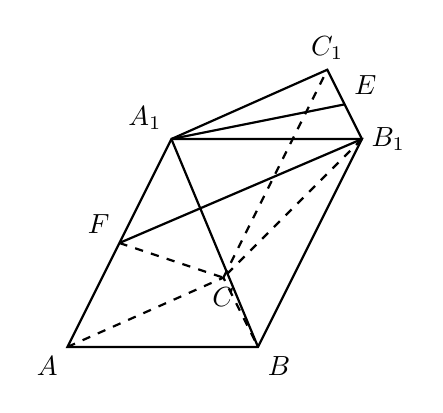
\begin{tikzpicture}[>=stealth, scale=1.1]
  % 底面顶点
  \coordinate (A) at (0, 0);
  \coordinate (B) at (2.2, 0);
  \coordinate (C) at (1.8, 0.8);

  % 侧棱向量: (1.2, 2.4)
  \coordinate (A1) at (1.2, 2.4);
  \coordinate (B1) at (3.4, 2.4);
  \coordinate (C1) at (3.0, 3.2);

  % 中点 F on A1A, E on B1C1
  \coordinate (F) at (0.6, 1.2);
  \coordinate (E) at (3.2, 2.8);

  % 实线棱
  \draw[thick] (A) -- (B) -- (B1) -- (A1) -- cycle;
  \draw[thick] (A1) -- (C1) -- (B1);
  \draw[thick] (A1) -- (B);
  \draw[thick] (A1) -- (E);
  \draw[thick] (B1) -- (F);

  % 虚线棱与辅助线
  \draw[dashed, thick] (A) -- (C) -- (B);
  \draw[dashed, thick] (C) -- (C1);
  \draw[dashed, thick] (F) -- (C);
  \draw[dashed, thick] (B1) -- (C);

  % 顶点标签
  \node[below left] at (A) {$A$};
  \node[below right] at (B) {$B$};
  \node[below] at (C) {$C$};
  \node[above left] at (A1) {$A_1$};
  \node[right] at (B1) {$B_1$};
  \node[above] at (C1) {$C_1$};
  \node[above left] at (F) {$F$};
  \node[above right] at (E) {$E$};
\end{tikzpicture}
\end{center}
\nopagebreak[4]
\Needspace{4\baselineskip}
\textbf{解析}

\textbf{(1)}
设 $A_1$ 在底面 $ABC$ 上的射影为 $O$．
连接 $A_1O$，则 $A_1O \perp \text{\text{平面} } ABC$．
作 $A_1H_1 \perp AB$ 于 $H_1$，$A_1H_2 \perp AC$ 于 $H_2$．
由三垂线定理的逆定理知 $OH_1 \perp AB, OH_2 \perp AC$．
在 $\text{Rt}\triangle A_1AH_1$ 与 $\text{Rt}\triangle A_1AH_2$ 中，$A_1A$ 为公共斜边，且 $\angle A_1AB = \angle A_1AC$．
所以 $\text{Rt}\triangle A_1AH_1 \cong \text{Rt}\triangle A_1AH_2$，$A_1H_1 = A_1H_2$．
进而 $OH_1 = OH_2$，说明射影 $O$ 在 $\angle BAC$ 的平分线所在直线上．
取 $BC$ 的中点 $D$，连接 $AD$．因为 $AB = AC$，所以 $AD \perp BC$ 且 $AD$ 是 $\angle BAC$ 的平分线，故点 $O$ 落在直线 $AD$ 上．
因此 $A_1A$ 与底面 $ABC$ 所成的角即为 $\angle A_1AD$．
又侧面 $B_1BCC_1$ 与底面 $ABC$ 所成的二面角为 $120^\circ$，其平面角为钝角，
由几何关系可推得 $\angle A_1AD = 60^\circ$．
故 $A_1A$ 与底面 $ABC$ 所成的角为 $60^\circ$．

\textbf{(2)}
取 $BC$ 的中点 $D$，连接 $A_1D, B_1D$．
因为 $E$ 是 $B_1C_1$ 的中点，在平行四边形 $B_1BCC_1$ 中，侧棱平行且相等，中点连线与侧棱平行，
取 $B_1C$ 的中点 $M$，连接 $FM, ME$．
在 $\triangle A_1AC$ 中，$F$ 是 $A_1A$ 的中点，$M$ 是 $B_1C$ 与平行对角线的交点，
\Needspace{5\baselineskip}
通过向量关系表示：
\nopagebreak[4]
\[
\vec{A_1E} = \vec{A_1B_1} + \vec{B_1E} = \vec{AB} + \dfrac{1}{2}\vec{B_1C_1}.
\]
而在平面 $B_1FC$ 中，利用平行四边形中位线平行关系可知 $A_1E$ 平行于平面 $B_1FC$ 内的中线．
又 $A_1E \not\subset \text{\text{平面} } B_1FC$，
所以 $A_1E \parallel \text{\text{平面} } B_1FC$．

\textbf{(3)}
经过 $A_1, A, B, C$ 四点的球即三棱锥 $A_1-ABC$ 的外接球．
由 (1) 知 $A_1A = a$，底面与侧棱对称性质可得球心位于对称垂线上．
\Needspace{5\baselineskip}
设球的半径为 $R$，由高与截面圆半径关系计算得：
\nopagebreak[4]
\[
R = \dfrac{\sqrt{3}}{3} a.
\]
\Needspace{5\baselineskip}
经过四点的球的体积为：
\nopagebreak[4]
\[
V = \dfrac{4}{3} \pi R^3 = \dfrac{4}{3} \pi \left(\dfrac{\sqrt{3}}{3} a\right)^3 = \dfrac{4\sqrt{3}}{27} \pi a^3.
\]

\gkanswer{答案（1）：$A_1A$ 与底面 $ABC$ 所成的角为 $60^\circ$（或 $\dfrac{\pi}{3}$）。}

\gkanswer{答案（2）：见解析版}

\gkanswer{答案（3）：$\dfrac{4\sqrt{3}}{27}\pi a^3$。}

\end{answer}
\begin{answer}
\gksolhead{20}{}

\textbf{题目}：

某人在一山坡 $P$ 处观看对面山顶上的一座铁塔，如图所示，塔高 $BC = 80$ 米，塔所在的山高 $OB = 220$ 米，$OA = 200$ 米，图中所示的山坡可视为直线 $l$ 且点 $P$ 在直线 $l$ 上，$l$ 与水平地面的夹角为 $\alpha$，$\tan \alpha = \dfrac{1}{2}$．试问此人距水平地面多高时，观看塔的视角 $\angle BPC$ 最大？（不计此人的身高）
\nopagebreak[4]
\begin{center}\begin{tikzpicture}[>=stealth, scale=0.85]
  % 基准坐标
  \coordinate (O) at (0, 0);
  \coordinate (A) at (2.0, 0);
  \coordinate (B) at (0, 2.6);
  \coordinate (C) at (0, 3.5);
  \coordinate (P) at (3.8, 0.9);

  % 水平地面虚线
  \draw[dashed, thick] (O) -- (5.6, 0) node[right] {水平地面};
  % 山高 OB 虚线
  \draw[dashed, thick] (O) -- (B);

  % 铁塔 BC
  \draw[thick] (-0.15, 2.6) -- (0.15, 2.6) -- (0, 3.5) -- cycle;

  % 山坡 l 射线
  \draw[thick] (A) -- (5.4, 1.7) node[above right] {$l$ (山坡)};

  % 视线 PB, PC
  \draw[thick] (P) -- (B);
  \draw[thick] (P) -- (C);

  % 坡角 alpha 标注
  \draw (2.7, 0) arc (0:26.565:0.7);
  \node at (2.9, 0.2) {$\alpha$};

  % 顶点标签
  \node[below left] at (O) {$O$};
  \node[left] at (B) {$B$};
  \node[above] at (C) {$C$};
  \node[below] at (A) {$A$};
  \node[below right] at (P) {$P$};
\end{tikzpicture}
\end{center}
\nopagebreak[4]
\Needspace{4\baselineskip}
\textbf{解析}

以山底水平地面 $O$ 点为原点，水平向右为 $x$ 轴正方向，竖直向上为 $y$ 轴正方向建立平面直角坐标系．
由题意：
\begin{itemize}
\item 塔所在的山高 $OB = 220$ 米，塔高 $BC = 80$ 米，
\end{itemize}
  所以塔底点 $B$ 的坐标为 $(0, 220)$，塔顶点 $C$ 的坐标为 $(0, 300)$．
\begin{itemize}
\item 山坡起点 $A$ 的坐标为 $(200, 0)$．
\item 山坡的坡角为 $\alpha$，且 $\tan \alpha = \dfrac{1}{2}$．
\end{itemize}
设观察点 $P$ 距水平地面的高度为 $h$ 米（$h > 0$）．
点 $P$ 在直线 $l$ 上，点 $P$ 到点 $A$ 的水平距离为 $\dfrac{h}{\tan \alpha} = 2h$．
因此点 $P$ 的坐标为 $(200 + 2h, h)$．

\Needspace{5\baselineskip}
在平面直角坐标系中，计算向量 $\vec{PB}$ 与 $\vec{PC}$：
\nopagebreak[4]
\[
\vec{PB} = (-200 - 2h, 220 - h),
\]
\nopagebreak[4]
\[
\vec{PC} = (-200 - 2h, 300 - h).
\]
\Needspace{5\baselineskip}
根据向量夹角公式或正切差角公式，视角 $\angle BPC = \theta$ 满足：
\nopagebreak[4]
\[
\tan \theta = \left|\dfrac{k_{PC} - k_{PB}}{1 + k_{PC}k_{PB}}\right| = \dfrac{\vec{PB} \times \vec{PC} \text{（\text{行列式}）}}{\vec{PB} \cdot \vec{PC}}.
\]
\Needspace{5\baselineskip}
分子为二维叉积（即三角形有向面积的 $2$ 倍）：
\nopagebreak[4]
\[
\begin{aligned}
(-200 - 2h)(300 - h) - (220 - h)(-200 - 2h) &= (200 + 2h)[-(300 - h) + (220 - h)] \\
&= (200 + 2h)(-80).
\end{aligned}
\]
取绝对值后分子为 $80(200 + 2h) = 160(h + 100)$．
\Needspace{5\baselineskip}
分母为向量数量积：
\nopagebreak[4]
\[
\begin{aligned}
\vec{PB} \cdot \vec{PC} &= (-200 - 2h)^2 + (220 - h)(300 - h) \\
&= 4(h + 100)^2 + (h^2 - 520h + 66000) \\
&= 4h^2 + 800h + 40000 + h^2 - 520h + 66000 \\
&= 5h^2 + 280h + 106000.
\end{aligned}
\]
\Needspace{5\baselineskip}
因此：
\nopagebreak[4]
\[
\tan \theta = \dfrac{160(h + 100)}{5h^2 + 280h + 106000}.
\]
令 $t = h + 100$（$t > 100$），则 $h = t - 100$．
\Needspace{5\baselineskip}
将 $h$ 代入分母：
\nopagebreak[4]
\[
\begin{aligned}
5(t - 100)^2 + 280(t - 100) + 106000 &= 5(t^2 - 200t + 10000) + 280t - 28000 + 106000 \\
&= 5t^2 - 1000t + 50000 + 280t + 78000 \\
&= 5t^2 - 720t + 128000.
\end{aligned}
\]
\Needspace{5\baselineskip}
故：
\nopagebreak[4]
\[
\tan \theta = \dfrac{160t}{5t^2 - 720t + 128000} = \dfrac{160}{5t + \dfrac{128000}{t} - 720}.
\]
\Needspace{5\baselineskip}
由基本不等式，当且仅当 $5t = \dfrac{128000}{t}$ 时，分母取得最小值，此时 $\tan \theta$ 取得最大值：
\nopagebreak[4]
\[
5t^2 = 128000 \implies t^2 = 25600 \implies t = 160.
\]
\Needspace{5\baselineskip}
因为 $t = h + 100$，所以：
\nopagebreak[4]
\[
h = t - 100 = 160 - 100 = 60 \text{（\text{米}）}.
\]
故当此人距水平地面 $60$ 米时，观看塔的视角 $\angle BPC$ 最大．

\gkanswer{答案：此人距水平地面 $60$ 米时，观看塔的视角 $\angle BPC$ 最大。}

\end{answer}
\begin{answer}
\gksolhead{21}{}

\textbf{题目}：

抛物线 $C$ 的方程为 $y = ax^2\ (a < 0)$，过抛物线 $C$ 上一点 $P(x_0, y_0)\ (x_0 \neq 0)$ 作斜率为 $k_1, k_2$ 的两条直线分别交抛物线 $C$ 于 $A(x_1, y_1), B(x_2, y_2)$ 两点（$P, A, B$ 三点互不相同），且满足 $k_2 + \lambda k_1 = 0\ (\lambda \neq 0, \lambda \neq -1)$．

(1) 求抛物线 $C$ 的焦点坐标和准线方程；

(2) 设直线 $AB$ 上一点 $M$，满足 $\vec{BM} = \lambda \vec{MA}$，证明线段 $PM$ 的中点在 $y$ 轴上；

(3) 当 $\lambda = 1$ 时，若点 $P$ 的坐标为 $(1, -1)$，求 $\angle PAB$ 为钝角时点 $A$ 的纵坐标 $y_1$ 的取值范围．

\Needspace{4\baselineskip}
\textbf{解析}

\textbf{(1)}
\Needspace{5\baselineskip}
抛物线方程为 $y = ax^2$（$a < 0$），改写为标准方程形式：
\nopagebreak[4]
\[
x^2 = \dfrac{1}{a} y.
\]
其焦点在 $y$ 轴负半轴上，开口向下，标准参数 $2p = -\dfrac{1}{a}$，即 $\dfrac{p}{2} = -\dfrac{1}{4a}$．
因此抛物线 $C$ 的焦点坐标为 $\left(0, \dfrac{1}{4a}\right)$，准线方程为 $y = -\dfrac{1}{4a}$．

\textbf{(2)}
设点 $P(x_0, y_0)$，$A(x_1, y_1)$，$B(x_2, y_2)$ 均在抛物线 $y = ax^2$ 上．
\Needspace{5\baselineskip}
直线 $PA$ 的斜率为：
\nopagebreak[4]
\[
k_1 = \dfrac{y_1 - y_0}{x_1 - x_0} = \dfrac{a(x_1^2 - x_0^2)}{x_1 - x_0} = a(x_1 + x_0).
\]
\Needspace{5\baselineskip}
直线 $PB$ 的斜率为：
\nopagebreak[4]
\[
k_2 = \dfrac{y_2 - y_0}{x_2 - x_0} = \dfrac{a(x_2^2 - x_0^2)}{x_2 - x_0} = a(x_2 + x_0).
\]
\Needspace{5\baselineskip}
已知 $k_2 + \lambda k_1 = 0$ 且 $a \neq 0$，代入得：
\nopagebreak[4]
\[
a(x_2 + x_0) + \lambda a(x_1 + x_0) = 0 \implies x_2 + \lambda x_1 + (1 + \lambda)x_0 = 0.
\]
因为点 $M$ 在直线 $AB$ 上且满足 $\vec{BM} = \lambda \vec{MA}$，
\Needspace{5\baselineskip}
由定比分点公式，点 $M$ 的横坐标为：
\nopagebreak[4]
\[
x_M = \dfrac{x_2 + \lambda x_1}{1 + \lambda}.
\]
\Needspace{5\baselineskip}
将 $x_2 + \lambda x_1 = -(1 + \lambda)x_0$ 代入可得：
\nopagebreak[4]
\[
x_M = \dfrac{-(1 + \lambda)x_0}{1 + \lambda} = -x_0.
\]
\Needspace{5\baselineskip}
因此线段 $PM$ 中点的横坐标为：
\nopagebreak[4]
\[
x_{\text{\text{中}}} = \dfrac{x_0 + x_M}{2} = \dfrac{x_0 + (-x_0)}{2} = 0.
\]
故线段 $PM$ 的中点在 $y$ 轴上．

\textbf{(3)}
当 $\lambda = 1$ 时，点 $P(1, -1)$ 在抛物线 $y = ax^2$ 上，代入得 $-1 = a(1)^2 \implies a = -1$．
抛物线方程为 $y = -x^2$．
\Needspace{5\baselineskip}
由 $\lambda = 1$ 且 $x_0 = 1$，条件 $x_2 + \lambda x_1 + (1 + \lambda)x_0 = 0$ 成为：
\nopagebreak[4]
\[
x_2 + x_1 + 2 = 0 \implies x_2 = -x_1 - 2.
\]
因为 $P, A, B$ 为互不相同的点：
$A \neq P \implies x_1 \neq 1$；
$B \neq P \implies x_2 \neq 1 \iff -x_1 - 2 \neq 1 \implies x_1 \neq -3$；
$A \neq B \implies x_1 \neq x_2 \iff x_1 \neq -x_1 - 2 \implies x_1 \neq -1$．
故 $x_1 \notin \{-3, -1, 1\}$．
各点坐标为 $P(1, -1)$，$A(x_1, -x_1^2)$，$B(-x_1-2, -(-x_1-2)^2)$．
\Needspace{5\baselineskip}
计算向量：
\nopagebreak[4]
\[
\vec{AP} = (1 - x_1, -1 - (-x_1^2)) = (1 - x_1, x_1^2 - 1) = (1 - x_1)(1, -(x_1 + 1)),
\]
\nopagebreak[4]
\[
\vec{AB} = (x_2 - x_1, -x_2^2 - (-x_1^2)) = (x_2 - x_1)(1, -(x_1 + x_2)).
\]
\Needspace{5\baselineskip}
将 $x_2 - x_1 = -2x_1 - 2 = -2(x_1 + 1)$ 及 $x_1 + x_2 = -2$ 代入：
\nopagebreak[4]
\[
\vec{AB} = -2(x_1 + 1)(1, 2).
\]
\Needspace{5\baselineskip}
$\angle PAB$ 为钝角的充要条件是 $\vec{AP}\cdot\vec{AB} < 0$ 且两向量不共线（三点在抛物线上显然不共线）：
\nopagebreak[4]
\[
\begin{aligned}
\vec{AP}\cdot\vec{AB} &= (1 - x_1)(-2(x_1 + 1))\Big[1 \times 1 + (-(x_1 + 1)) \times 2\Big] \\
&= -2(1 - x_1)(x_1 + 1)(1 - 2x_1 - 2) \\
&= -2(1 - x_1)(x_1 + 1)(-2x_1 - 1).
\end{aligned}
\]
\Needspace{5\baselineskip}
化简：
\nopagebreak[4]
\[
\vec{AP}\cdot\vec{AB} = 2(1 - x_1^2)(2x_1 + 1) = -2(x_1^2 - 1)(2x_1 + 1).
\]
\Needspace{5\baselineskip}
令 $\vec{AP}\cdot\vec{AB} < 0$：
\nopagebreak[4]
\[
-2(x_1^2 - 1)(2x_1 + 1) < 0 \iff (x_1^2 - 1)(2x_1 + 1) > 0 \iff (x_1 - 1)(x_1 + 1)(2x_1 + 1) > 0.
\]
\Needspace{5\baselineskip}
解此一元三次不等式，根为 $-1, -\dfrac{1}{2}, 1$：
\nopagebreak[4]
\[
-1 < x_1 < -\dfrac{1}{2} \quad \text{\text{或}} \quad x_1 > 1.
\]
（注意到 $-3, -1, 1$ 均不在该解集内，自然满足相异性）．
点 $A$ 的纵坐标为 $y_1 = -x_1^2$：
1. 当 $-1 < x_1 < -\dfrac{1}{2}$ 时，$x_1^2 \in \left(\dfrac{1}{4}, 1\right)$，则 $y_1 = -x_1^2 \in \left(-1, -\dfrac{1}{4}\right)$；
2. 当 $x_1 > 1$ 时，$x_1^2 \in (1, +\infty)$，则 $y_1 = -x_1^2 \in (-\infty, -1)$．
\Needspace{5\baselineskip}
综上所述，点 $A$ 的纵坐标 $y_1$ 的取值范围为：
\nopagebreak[4]
\[
(-\infty, -1) \cup \left(-1, -\dfrac{1}{4}\right).
\]

\gkanswer{答案（1）：焦点坐标为 $\left(0, \dfrac{1}{4a}\right)$，准线方程为 $y = -\dfrac{1}{4a}$。}

\gkanswer{答案（2）：见解析版}

\gkanswer{答案（3）：$y_1$ 的取值范围为 $(-\infty, -1) \cup \left(-1, -\dfrac{1}{4}\right)$。}

\end{answer}
\begin{answer}
\gksolhead{22}{}

\textbf{题目}：

设函数 $f(x) = x \sin x\ (x \in \mathbf{R})$．

(1) 证明 $f(x + 2k\pi) - f(x) = 2k\pi \sin x$，其中 $k$ 为整数；

(2) 设 $x_0$ 为 $f(x)$ 的一个极值点，证明 $[f(x_0)]^2 = \dfrac{x_0^4}{1 + x_0^2}$；

(3) 设 $f(x)$ 在 $(0, +\infty)$ 内的全部极值点按从小到大的顺序排列为 $a_1, a_2, \cdots, a_n, \cdots$，证明 $\dfrac{\pi}{2} < a_{n+1} - a_n < \pi\ (n = 1, 2, \cdots)$．

\Needspace{4\baselineskip}
\textbf{解析}

\textbf{(1)}
对任意整数 $k \in \mathbf{Z}$，由正弦函数的周期性知 $\sin(x + 2k\pi) = \sin x$．
\Needspace{5\baselineskip}
因此：
\nopagebreak[4]
\[
\begin{aligned}
f(x + 2k\pi) &= (x + 2k\pi) \sin(x + 2k\pi) \\
&= (x + 2k\pi) \sin x \\
&= x \sin x + 2k\pi \sin x \\
&= f(x) + 2k\pi \sin x.
\end{aligned}
\]
\Needspace{5\baselineskip}
移项即得：
\nopagebreak[4]
\[
f(x + 2k\pi) - f(x) = 2k\pi \sin x.
\]

\textbf{(2)}
\Needspace{5\baselineskip}
函数 $f(x) = x \sin x$ 在 $\mathbf{R}$ 上可导，求导得：
\nopagebreak[4]
\[
f'(x) = \sin x + x \cos x.
\]
\Needspace{5\baselineskip}
若 $x_0$ 为 $f(x)$ 的一个极值点，由费马引理知 $f'(x_0) = 0$，即：
\nopagebreak[4]
\[
\sin x_0 + x_0 \cos x_0 = 0 \implies \sin x_0 = -x_0 \cos x_0.
\]
若 $\cos x_0 = 0$，则由上式得 $\sin x_0 = 0$，与 $\sin^2 x_0 + \cos^2 x_0 = 1$ 矛盾，
故 $\cos x_0 \neq 0$．
\Needspace{5\baselineskip}
等式两边同除以 $\cos x_0$，得：
\nopagebreak[4]
\[
\tan x_0 = -x_0.
\]
\Needspace{5\baselineskip}
由同角三角函数的基本关系式：
\nopagebreak[4]
\[
\sin^2 x_0 = \dfrac{\tan^2 x_0}{1 + \tan^2 x_0} = \dfrac{(-x_0)^2}{1 + (-x_0)^2} = \dfrac{x_0^2}{1 + x_0^2}.
\]
\Needspace{5\baselineskip}
因此：
\nopagebreak[4]
\[
[f(x_0)]^2 = (x_0 \sin x_0)^2 = x_0^2 \sin^2 x_0 = x_0^2 \cdot \dfrac{x_0^2}{1 + x_0^2} = \dfrac{x_0^4}{1 + x_0^2}.
\]
结论获证．

\textbf{(3)}
由 (2) 知，$f(x)$ 在 $(0, +\infty)$ 内的极值点满足超越方程 $\tan x = -x$．
考虑函数 $g(x) = \tan x + x$：
\begin{itemize}
\item 在开区间 $I_n = \left(n\pi - \dfrac{\pi}{2}, n\pi\right)$（$n = 1, 2, \cdots$）内：
\end{itemize}
  $g'(x) = \sec^2 x + 1 > 0$，函数 $g(x)$ 严格单调递增；
  端点极限 $\lim\limits_{x \to (n\pi - \frac{\pi}{2})^+} g(x) = -\infty$，$g(n\pi) = 0 + n\pi = n\pi > 0$．
  由零点存在性定理与单调性，函数 $g(x)$ 在区间 $I_n$ 内有且仅有一个零点，记为 $a_n$．
\begin{itemize}
\item 在区间 $\left[n\pi, n\pi + \dfrac{\pi}{2}\right)$ 内：
\end{itemize}
  当 $x \in [n\pi, n\pi + \frac{\pi}{2})$ 时，$\tan x \geqslant 0$，而 $x > 0$，所以 $\tan x + x > 0$，无零点．
\begin{itemize}
\item 当 $x \in \left(0, \dfrac{\pi}{2}\right)$ 时，$\tan x > 0, x > 0$，亦无零点．
\item 当 $x = k\pi + \dfrac{\pi}{2}$ 时，$\cos x = 0$，$f'(x) = \sin x = \pm 1 \neq 0$，非极值点．
\end{itemize}
\Needspace{5\baselineskip}
因此，$f(x)$ 在 $(0, +\infty)$ 内的全部极值点按从小到大依次排列为 $a_1, a_2, \cdots, a_n, \cdots$，且满足：
\nopagebreak[4]
\[
n\pi - \dfrac{\pi}{2} < a_n < n\pi \quad (n = 1, 2, \cdots).
\]

现证明不等式 $\dfrac{\pi}{2} < a_{n+1} - a_n < \pi$：

① 先证左半边 $a_{n+1} - a_n > \dfrac{\pi}{2}$：
\Needspace{5\baselineskip}
由上述范围，对第 $n+1$ 个极值点：
\nopagebreak[4]
\[
(n+1)\pi - \dfrac{\pi}{2} < a_{n+1} < (n+1)\pi,
\]
即 $n\pi + \dfrac{\pi}{2} < a_{n+1}$．
而 $a_n < n\pi \implies -a_n > -n\pi$．
\Needspace{5\baselineskip}
两式相加即得：
\nopagebreak[4]
\[
a_{n+1} - a_n > \left(n\pi + \dfrac{\pi}{2}\right) - n\pi = \dfrac{\pi}{2}.
\]

② 再证右半边 $a_{n+1} - a_n < \pi$：
由定义，$\tan a_n = -a_n$，$\tan a_{n+1} = -a_{n+1}$．
\Needspace{5\baselineskip}
因为正切函数的周期为 $\pi$，所以：
\nopagebreak[4]
\[
\tan(a_n + \pi) = \tan a_n = -a_n.
\]
因为 $n\pi - \dfrac{\pi}{2} < a_n < n\pi$，
所以 $(n+1)\pi - \dfrac{\pi}{2} < a_n + \pi < (n+1)\pi$．
这表明 $a_{n+1}$ 与 $a_n + \pi$ 都落在同一个正切函数的单调递增区间 $\left((n+1)\pi - \dfrac{\pi}{2}, (n+1)\pi\right)$ 内．
因为数列 $\{a_n\}$ 严格递增，$a_{n+1} > a_n > 0$，
\Needspace{5\baselineskip}
所以 $-a_{n+1} < -a_n$，即：
\nopagebreak[4]
\[
\tan a_{n+1} < \tan(a_n + \pi).
\]
由于函数 $y = \tan x$ 在区间 $\left((n+1)\pi - \dfrac{\pi}{2}, (n+1)\pi\right)$ 内严格单调递增，
\Needspace{5\baselineskip}
由函数值的单调性必有自变量的不等关系：
\nopagebreak[4]
\[
a_{n+1} < a_n + \pi \implies a_{n+1} - a_n < \pi.
\]

\Needspace{5\baselineskip}
综合 ① 与 ②，得：
\nopagebreak[4]
\[
\dfrac{\pi}{2} < a_{n+1} - a_n < \pi \quad (n = 1, 2, \cdots).
\]
证毕．

\gkanswer{答案（1）：见解析版}

\gkanswer{答案（2）：见解析版}

\gkanswer{答案（3）：见解析版}

\end{answer}